\documentclass[10pt, twocolumn]{article}
\usepackage[margin=1in]{geometry}
\usepackage{graphicx}
\usepackage{microtype}
\usepackage{verbatim}
\usepackage{amsmath}
\usepackage{nicefrac}
\usepackage[colorlinks=false, hidelinks]{hyperref}
\usepackage{caption}
\usepackage{subcaption}
\usepackage{listings}

\title{%
	\makebox[\textwidth][s]{%
		\hfill
		\begin{tabular}[b]{@{}c@{}}
				\fontsize{14}{20}\bfseries\selectfont \emph{Easy--PCB} Solder Reflow Oven\\
				\fontsize{12}{18}\selectfont Ben Lorenzetti\\
 		\end{tabular}%
    		\hfill
    		\makebox[0pt][r]{%
      			\includegraphics[width=0.2\textwidth]{Figures/easy-pcb-oven.pdf}}%
 	}% end makebox
}% end title

\author{}
\date{}

\begin{document}

\maketitle

\section*{Features}
\addcontentsline{toc}{section}{Features}

\begin{flushleft}
	\begin{itemize}
		\fontsize{10}{12}\bfseries\selectfont
		\item Insulated aluminum frame with XxYxZ interior chamber
		\item XXX Watt heating element with solid state relay control
		\item Forced convection fan driven by bipolar stepper motor with speed control
		\item Type X thermocouple for temperature feedback loop
		\item XXXXX based feedback control
		\item Integrated 120 VAC power supply with surge and short protection
		\item Combined temperature/run time \mbox{7--segment} display
		\item Convenient pushbutton/menu interface for temperature profile programming
	\end{itemize}
\end{flushleft}

\section*{Introduction}
\addcontentsline{toc}{section}{Introduction}

\emph{Easy--PCB} is a small, desktop convection oven for DIY reflow soldering at home.

As integrated circuits continue to become smaller and faster,
many $\mu$--controllers, FPGAs, and other ICs are no longer available in
DIP form for breadboard prototyping or solder iron soldering.
Similar to the shift away from PC parallel ports in the early 2000s,
the shift away from DIPs means modern electronics hobbyists need more
complicated equipment than their predessesors.

Currently, commercial solder reflow stations are available for
soldering fine pitch, SMD, and BGA componenets.
More recently, several hackers have created open source designs
for inexpensive reflow ovens, using converted kitchen toaster ovens.

\emph{Easy--PCB} is better because it is a convection oven;
controlled air flow prevents parts from being blown out of position and
convection heating obviates the uneven heat absorbtion seen in infrared radiation based systems.
Furthermore, \emph{Easy--PCB} was designed from the ground up for soldering,
so the heating elements and oven frame were optimized alongside the
temperature controller for a typical solder reflow profile.

\begin{center}
	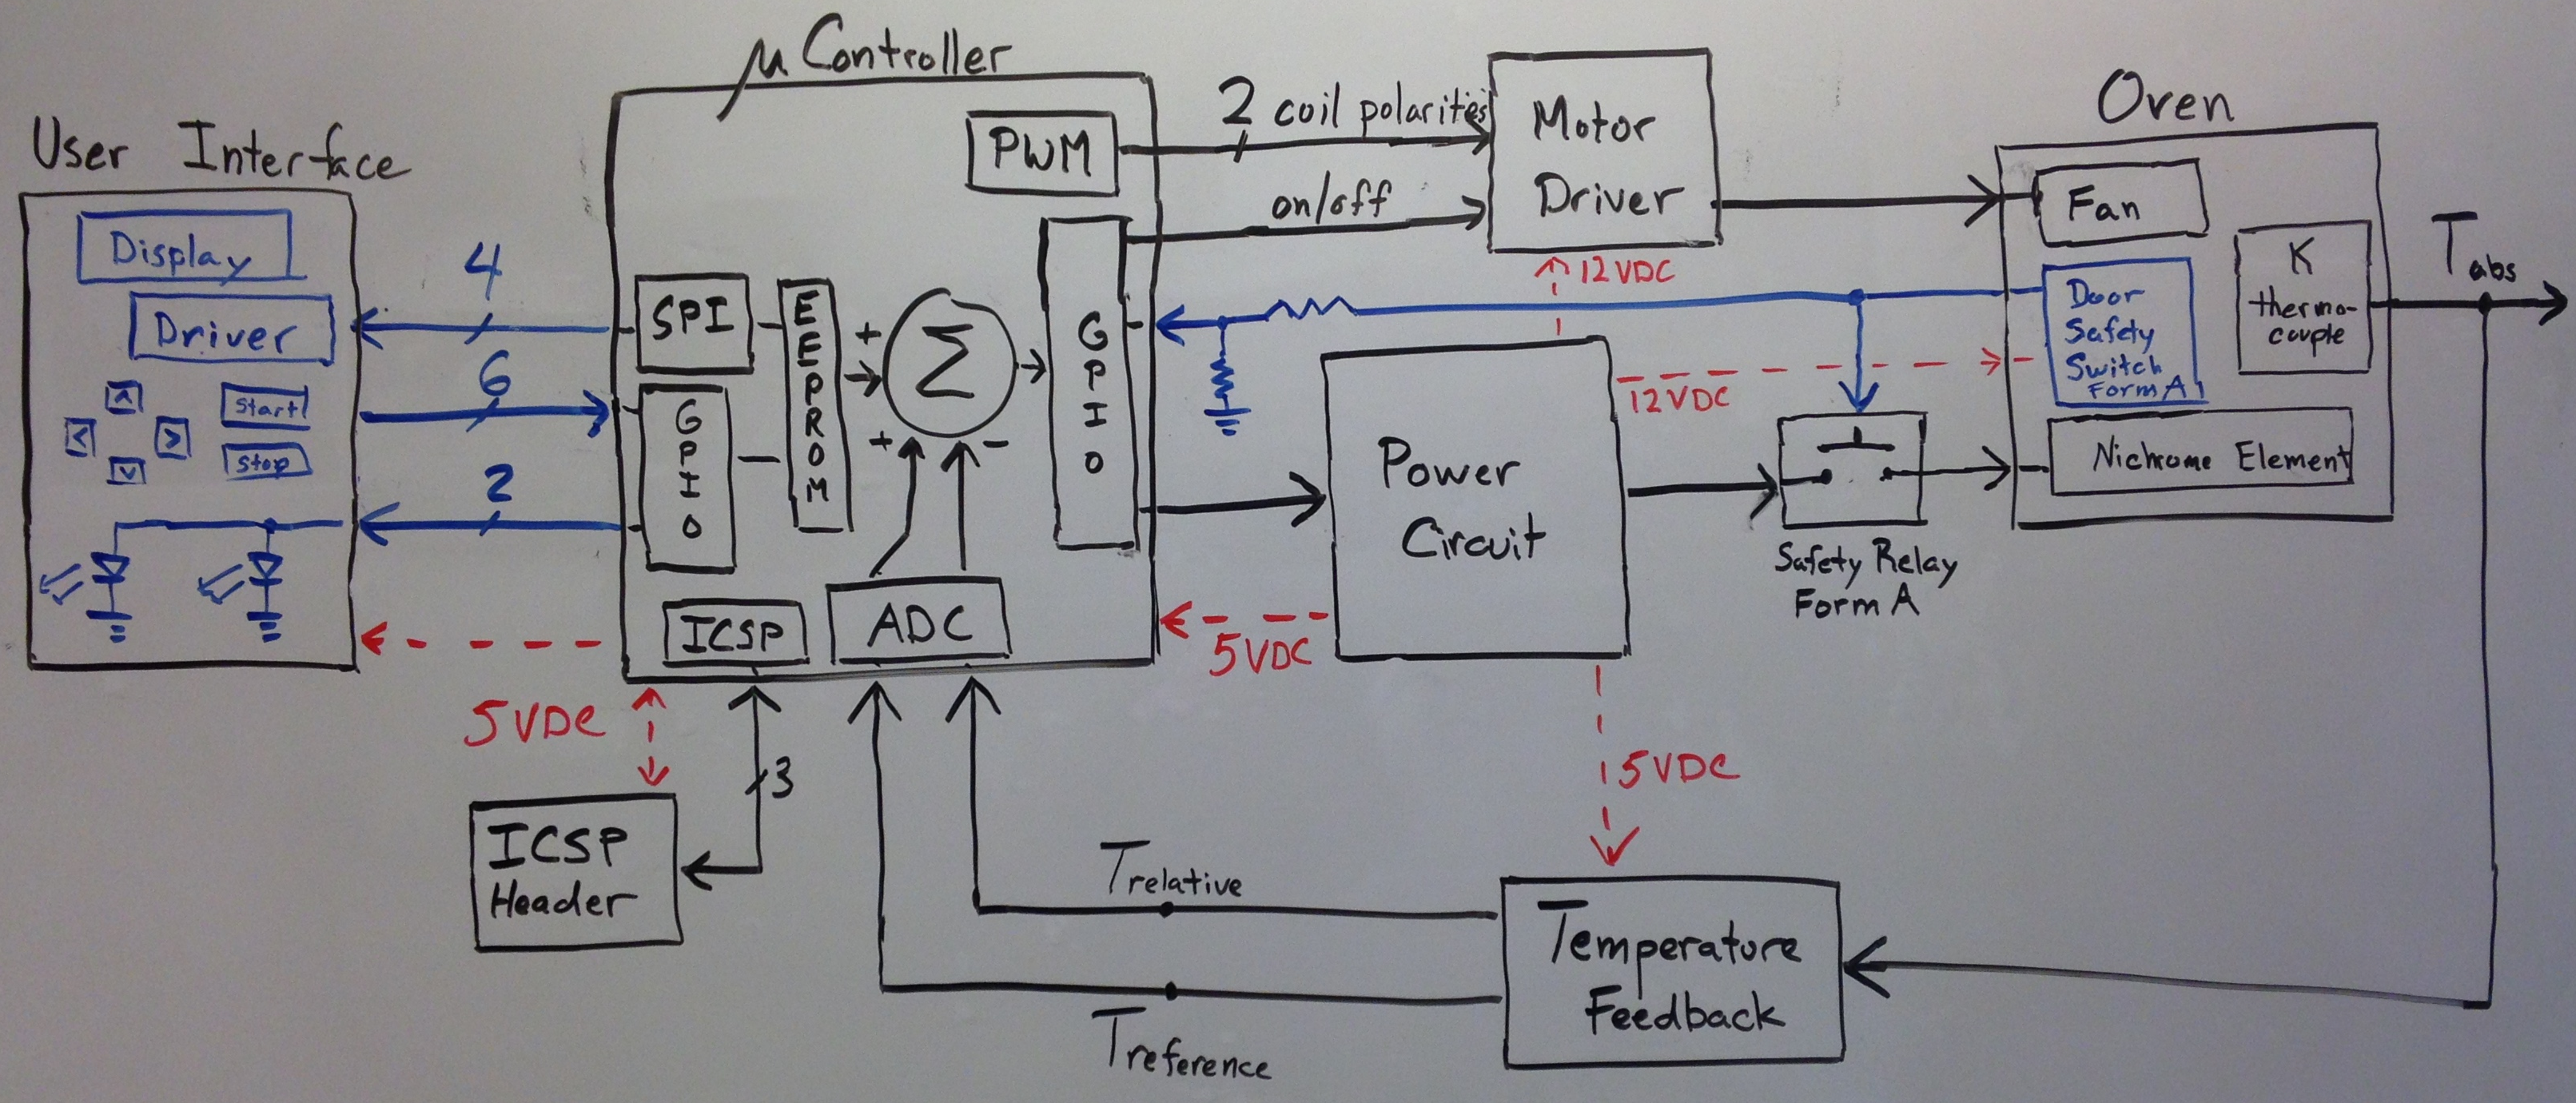
\includegraphics[width=\columnwidth]{Figures/control-system.pdf}
	\captionof*{figure}{The \emph{Easy--PCB} Control System: not just a controller bolted onto a disjoint oven.}
\end{center}

\emph{Easy--PCB} allows hobbyists to produce solder reflow temperature profiles with
a high degree of accuracy and repeatability.
Alongside freely available PCB design programs like Eagle and low-quantity
fabrication services like OSH Park, \emph{Easy--PCB} makes
modern integrated components, such as digital CMOS cameras,
within the range of capabilities of independent hobbyists.

\begin{center}
	\includegraphics[width=\columnwidth]{Figures/control-results.pdf}
	\captionof*{figure}{Faithful Temperature Profile Control}
\end{center}

\tableofcontents

\section{User Interface}

\section{Oven Design}


\end{document}
